\section{运动和静止}\label{sec:3-1}

我们经常可以看到,人在行走,汽车在行驶,河水在流动,轮船在航行,飞机在飞翔,我们说这些物体都在运动。
另一方面我们又看到房屋、桥梁、树木、山岭等总是在它原来的地方,我们说这些物体是静止的。
可是,地球在自转,同时还绕太阳公转,房屋、桥梁、树木、山岭等是固定在地球上的,所以它们也随着地球一起运动。
太阳也不是不动的,它和其它恒星一样,在银河系里运动。就是银河系,也在运动。
整个宇宙就是由运动着的物质组成的,绝对不动的物体是没有的。

既然一切物体都在运动,那么,我们平常说的这个物体在运动,那个物体是静止的,又是什么意思呢?

一辆公共汽车,如果它离车站的距离越来越远或越来越近,它对车站的位置在不断变化,我们就说它在运动。
如果这辆公共汽车对车站的位置不变,我们就说它是静止的。
可见,我们是根据公共汽车对车站的位置是否在改变,来判断它是运动还是静止的。
一般说来,我们\CJKunderwave{研究任何物体是否运动和怎样运动的时候,总是要先选择一个假定为不动的物体,
看被研究的物体对于这个假定为不动的物体的位置是否变化,来判断被研究的物体是否在运动}。
想想看,当你说一个物体在运动或静止时,是不是总是无意中先假定某个物体是不动的?

在物理学中,我们\textbf{把一个物体相对于别的物体的位置改变叫做机械运动},
在研究机械运动的时候,事先假定为不动的物体叫做\textbf{参照物}。

参照物是可以任意选择的。一辆装满货物的卡车,在公路上行驶着。
坐在卡车上的人,选卡车作参照物,他看到货物对卡车的位置不变,他认为货物是静止的。
站在路旁的人,选路旁的建筑物作参照物,他看到货物对建筑物的位置在不断变化着,他认为货物是运动的。
可见,物体是运动还是静止,跟参照物的选择有关系。

参照物虽然可以任意选择,但是为了研究问题的方便,我们应该选择最合适的参照物。
通常,在研究地面上物体运动的时候,就选地面或在地面上静止的物体作参照物。
在研究火车厢里人的运动的时候,可以选火车厢作参照物。

从上面讲的可以知道,我们平常所说的运动和静止都是相对的,总是相对于我们假定为不动的参照物来说的。

\newpage

\nonumsection{阅读材料:伽利略论运动和静止的对性}


\begin{wrapfigure}[9]{r}{5cm}
    \centering
    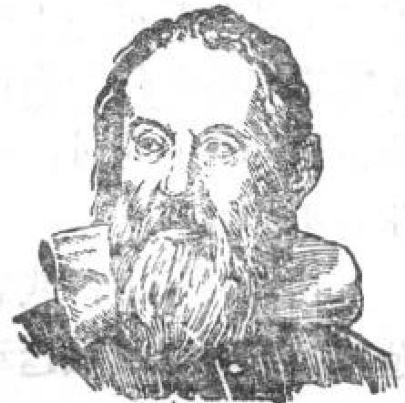
\includegraphics[width=4cm]{../pic/czwl1-ch3-a}
    \caption*{伽利略(1564 ~ 1642)}
\end{wrapfigure}

伟大的学者,近代物理学的奠基人,意大利的伽利略,第一个深刻地探讨了运动和静止的相对性,
生动地描述了不选定参照物就无法确定物体是否在运动。下面引用的是他的论述:

“把你和一些朋友关在一条大船甲板下的主舱里,再让你们带几只苍蝇、蝴蝶和其他小飞虫。
舱内放一只大水碗,其中放几条鱼。然后挂上一个水瓶,让水一滴一滴地滴到下面的一个宽口罐里。
船停着不动时,你留神观察,小虫都同等地向舱内各方面飞行,鱼向各个方向随便游动,水滴滴进下面的罐子中。
你把任何东西扔给你的朋友时,只要距离相等,向这一方向不必比另一方向用更多的力,你双脚齐跳,无论向哪个方向跳过的距离都相等。
当你仔细地观察这些事情后(虽然当船停止时,事情无疑一定是这样的),再使船以任何速度前进,只要运动是匀速的,也不忽左忽右地摆动。
你将发现,所有上述现象丝毫没有变化,你也无法从其中任何一个现象来确定,船是在运动还是停着不动。
即使船运动得相当快,在跳跃时,你将和以前一样,在船底板上跳过相同的距离,你跳向船尾也不会比跳向船头来得远,
虽然你跳到空中时,脚下的船底板向着你跳的相反方向移动。
你把不论什么东西扔给你的同伴时,不论他是在船头还是在船尾,只要你自己站在对面,你并不需要用更的力。
水滴将象先前一样,滴进下面的罐子,一滴也不会滴向船尾,虽然水滴在空中时,船已行驶了许多拃。
鱼在水中游向水碗前部所用的力,不比游向水碗后部来得大;它们一样悠闲地游向放在水碗边缘任何地方的食饵。
最后,蝴蝶和苍蝇将继续随便地到处飞行,它们也决不会向船尾集中,并不因为它们可能长时间留在空中,
脱离了船的运动,为赶上船的运动显出累的样子。
如果点香冒烟,则将看到烟象一朵云一样向上升起,不向任何一边飘动。”

